%Version 3 October 2023
% See section 11 of the User Manual for version history
%
%%%%%%%%%%%%%%%%%%%%%%%%%%%%%%%%%%%%%%%%%%%%%%%%%%%%%%%%%%%%%%%%%%%%%%
%%                                                                 %%
%% Please do not use \input{...} to include other tex files.       %%
%% Submit your LaTeX manuscript as one .tex document.              %%
%%                                                                 %%
%% All additional figures and files should be attached             %%
%% separately and not embedded in the \TeX\ document itself.       %%
%%                                                                 %%
%%%%%%%%%%%%%%%%%%%%%%%%%%%%%%%%%%%%%%%%%%%%%%%%%%%%%%%%%%%%%%%%%%%%%

%%\documentclass[referee,sn-basic]{sn-jnl}% referee option is meant for double line spacing

%%=======================================================%%
%% to print line numbers in the margin use lineno option %%
%%=======================================================%%

% \documentclass[lineno,sn-basic]{sn-jnl}% Basic Springer Nature Reference Style/Chemistry Reference Style

%%======================================================%%
%% to compile with pdflatex/xelatex use pdflatex option %%
%%======================================================%%

\documentclass[pdflatex,sn-basic, Numbered]{sn-jnl}

%%%% Standard Packages
%%<additional latex packages if required can be included here>

\usepackage{graphicx}%
\usepackage{multirow}%
\usepackage{amsmath,amssymb,amsfonts}%
\usepackage{amsthm}%
\usepackage{mathrsfs}%
\usepackage[title]{appendix}%
\usepackage{xcolor}%
\usepackage{textcomp}%
\usepackage{manyfoot}%
\usepackage{booktabs}%
\usepackage{algorithm}%
\usepackage{algorithmicx}%
\usepackage{algpseudocode}%
\usepackage{listings}%
\usepackage{multicol}

% additional packages
\usepackage{caption}
\usepackage{placeins}
\usepackage{lipsum}
\usepackage{float}
\usepackage{csquotes}
\usepackage{sidecap}
\usepackage{url}                     % fix URL wrap
\usepackage{booktabs}                % Improves the quality of tables in LaTeX
\usepackage{tabularx}                % Enhances the standard LaTeX tables
\usepackage{subcaption}              % Provides support for subfigures and subtables
\usepackage{longtable}               % Allows the creation of multi-page tables
\usepackage{multirow}                % Enables cells spanning multiple rows in tables
\usepackage{threeparttable}          % Provides additional functionality for tables
\usepackage{array}
\usepackage{eurosym}

\def\UrlBreaks{\do\/\do-}
\renewcommand{\floatpagefraction}{0.5}
\renewcommand{\textfraction}{0.1}

%% as per the requirement new theorem styles can be included as shown below
\theoremstyle{thmstyleone}%
\newtheorem{theorem}{Theorem}%  meant for continuous numbers
%%\newtheorem{theorem}{Theorem}[section]% meant for sectionwise numbers
%% optional argument [theorem] produces theorem numbering sequence instead of independent numbers for Proposition
\newtheorem{proposition}[theorem]{Proposition}%
%%\newtheorem{proposition}{Proposition}% to get separate numbers for theorem and proposition etc.

\theoremstyle{thmstyletwo}%
\newtheorem{example}{Example}%
\newtheorem{remark}{Remark}%
\theoremstyle{thmstylethree}%
\newtheorem{definition}{Definition}%

\raggedbottom
%%\unnumbered% uncomment this for unnumbered level heads

\newcommand{\comment}[1]{\textcolor{purple}{#1}}

%%=============================================================%%
%%=============================================================%%
\begin{document}

\title[Article Title]{24/7 carbon-free electricity matching accelerates adoption of advanced clean energy technologies}

%%=============================================================%%
%% GivenName	-> \fnm{Joergen W.}
%% Particle	-> \spfx{van der} -> surname prefix
%% FamilyName	-> \sur{Ploeg}
%% Suffix	-> \sfx{IV}
%% \author*[1,2]{\fnm{Joergen W.} \spfx{van der} \sur{Ploeg}
%%  \sfx{IV}}\email{iauthor@gmail.com}
%%=============================================================%%

\author*[1]{\fnm{Iegor} \sur{Riepin}}\email{iegor.riepin@tu-berlin.de}
\author[2]{\fnm{Jesse} \spfx{D.}  \sur{Jenkins}}\email{jessejenkins@princeton.edu}
\author[3]{\fnm{Devon} \sur{Swezey}}\email{dswezey@google.com}
\author[1]{\fnm{Tom} \sur{Brown}}\email{t.brown@tu-berlin.de}
\affil[1]{\orgdiv{Department of Digital Transformation in Energy Systems}, \orgname{TU Berlin}, \orgaddress{Germany}}
\affil[2]{\orgdiv{Mechanical \& Aerospace Engineering and Andlinger Center for Energy}, \orgname{Princeton University}, \orgaddress{USA}}
\affil[3]{\orgdiv{Global Energy and Climate}, \orgname{Google LLC}}

%%==================================%%
%% abstract %%
%%==================================%%

\abstract{

Commitments to 24/7 carbon-free energy matching by companies and governments create an early market for technologies that can fill the gaps between wind and solar generation.
We argue that the commitment by a small number of companies to round-the-clock matching can spur substantial learning in these advanced technologies.
We demonstrate these benefits for two technologies: long-duration energy storage and clean firm generation.
This makes 24/7 matching more attractive for other actors, leading to a virtuous circle that accelerates the time when the technologies become cost-competitive in the rest of the electricity market.
These indirect effects unlock greenhouse gas savings far beyond the direct emission reduction of initial investments.
}

%########################################################################
%########################################################################

\subsection*{Highlights}

\begin{itemize}
\item 24/7 CFE matching creates an early market for advanced electricity technologies
\item Early deployment of advanced technologies spurs substantial learning effect
\item Self-reinforcing system dynamics accelerate widespread adoption of advanced technologies
\item Indirect effects yield greenhouse gas savings far beyond the impact of initial investments
\end{itemize}


\subsection*{Abstract}
Commitments to 24/7 carbon-free energy matching by companies and governments create an early market for technologies that can fill the gaps between wind and solar generation.
We argue that the commitment by a small number of companies to round-the-clock matching can spur substantial learning in these advanced technologies.
We demonstrate these benefits for two technologies: long-duration energy storage and clean firm generation.
This makes 24/7 matching more attractive for other actors, leading to a virtuous circle that accelerates the time when the technologies become cost-competitive in the rest of the electricity market.
These indirect effects unlock greenhouse gas savings far beyond the direct emission reduction of initial investments.


\subsection*{Graphical abstract}

\begin{center}
    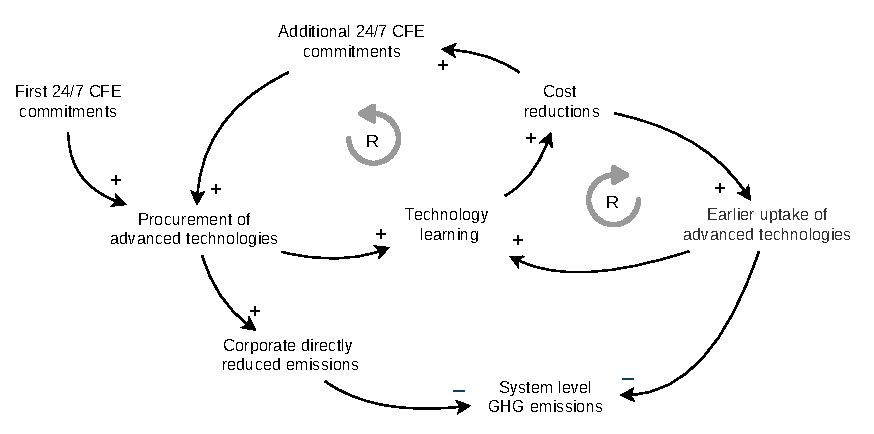
\includegraphics[width=0.85\textwidth]{images/virtuous_dynamics.pdf}
\end{center}


\subsection*{Metadata}
\begin{itemize}
    \item Words in text: 2706
    \item Words outside text (captions): 358
    \item Number of figures: 4
    \item Number of headers: 6
    \item Number of references: 20
    \item Supplementary information: Document S1. Table S1 (Technology assumptions) Supplementary references.
\end{itemize}


%########################################################################
%########################################################################

\maketitle

\subsection*{Big challenges ahead}\label{sec1}

Tackling climate change requires not only a massive scale-up of available energy technologies like wind, solar and batteries, but also an accelerated research, development, demonstration (RD\&D) and widespread deployment of advanced technologies that are not yet commercialised at scale \cite{sepulvedaRoleFirmLowCarbon2018, brownUltralongdurationEnergyStorage2023}.
Among them are clean firm generation technologies, such as next-generation geothermal power, advanced nuclear generators, Allam-cycle gas generators with carbon capture and storage (CCS), as well as long-duration energy storage (LDES) technologies, which can bridge multi-day gaps in clean power supply that cannot be filled by wind, solar photovoltaics (PV), or batteries.

\textbf{Barriers to commercialization---} Bringing new technologies to market on a large scale and in time, however, is fraught with challenges.
New technologies often face a \enquote{valley of death} on the path to successful commercial deployment \cite{google-advancedtech}.
Companies developing a new technology must first prove that it works safely and reliably at pilot scale.
One major hurdle at this stage is the scarcity of financing. Early-stage investments typically comprise R\&D grants and venture capital, insufficient in both magnitude and duration to support new energy technologies. On the other hand, mature technologies such as wind and solar attract steady, de-risked capital from institutional investors \cite{khatcherianBarriersTimelyDeployment2022}.

After that, companies must construct larger plants at sufficient scale and manufacturing cost to achieve commercial viability. This requires overcoming financial, engineering, and supply chain issues that come with building a first-of-its-kind (FOAK) project, and afterward optimizing processes to gradually cut the costs. Technology innovators frequently lack the expertise to scale from small demonstration plants to commercial-scale projects. Often, moving through this milestone requires a consortium of stakeholders, increasing project complexity and risk, thereby complicating financing \cite{google-advancedtech}.
Even when FOAK technologies are successfully demonstrated, scaling to subsequent projects remains difficult. New technologies must be repeatedly deployed to achieve economies of scale and reduce costs. However, procurement typically focuses on individual plants rather than larger portfolios, with many observers preferring to \enquote{wait and see} how the new generation of a technology performs before committing to an investment. Overall, the road from the first demonstration plant to commercial uptake can be complicated, risky, and expensive---and it is challenging to secure the capital to fund it.

\textbf{Bridging the valley of death---} Consider how solar became global industry and a truly disruptive technology. Bell Labs developed the first silicon photovoltaic cell in 1954, which made modern solar power possible. After more than 20 years of further development, in 1975, the Levelised Cost of Electricity (LCOE) for solar PV was above \$10,000/MWh in today's money. A historical trajectory for solar development involved Japan's niche markets for consumer electronics in the 1980s, and Germany's feed-in tariff in 2004, which created a \enquote{demand pull} leading to massive industrialization of solar PV manufacturing in China and rapid cost reduction through technological learning \cite{nemetHowSolarEnergy2019}. If we fast forward to 2020s, for projects with low-cost financing that tap high-quality resources, solar PV has now the cheapest levelised cost of electricity in history, with new utility-scale solar projects cost at \$30-60/MWh in Europe and the US and just \$20-40/MWh in China and India \cite{WorldEnergyOutlook2020}.

However, it took six decades for solar to become economically viable. The urgency of the climate crisis demands that we accelerate this process for advanced clean electricity technologies. A crucial question here: Who will invest in these technologies when they are expensive at the beginning? Understanding the wider social benefit of such investments is another important aspect.  New technologies, such as Allam cycle generators and iron-air battery storage are also likely to experience cost reductions through evolving R\&D process, learning by doing and iterative upscaling. In this way, even though initial investments come with a price premium and certain risks, they can result in cost reductions and an earlier rollout of advanced clean energy technologies. This produces indirect effects that result in greenhouse gas savings beyond the direct reductions associated with initial investments. The key is initial investments to start this process.

In this perspective, we illustrate in the following sections how initial commitments to 24/7 Carbon-Free Energy (CFE) matching can unlock these effects.

\subsection*{The significance of 24/7 CFE matching}\label{sec2}

Many public and private energy buyers are supporting the global effort to decarbonise electricity systems by purchasing clean energy.
An increasing number of buyers are adopting the most ambitious approach to clean energy purchasing, aiming to eliminate carbon emissions associated with their electricity use.
This approach is called the 24/7~CFE matching, i.e., aligning electricity demand with carbon-free energy energy supply on \textit{an hourly basis} and on the same local grid where demand occurs.
24/7~CFE commitments were announced by large technology companies such as Google, Microsoft and IronMountain, as well as by utilities, and the US federal government \cite{gocarbonfree247}.
% In 2021, an international group of stakeholders launched the 24/7 Carbon-free Energy Compact \cite{gocarbonfree247}. With over 150 signatories, the group aims to develop and scale high-impact technologies, energy policies, procurement practices, and solutions to make 24/7 Carbon-Free Energy achievable for all.

Motivated by these commitments, several quantitative studies have been conducted on the means, costs, and system-level impacts of hourly CFE matching \cite{xu-247CFE-report, ieaAdvancingDecarbonisationClean2022, riepinMeansCostsSystemlevel2024}. There are three key findings that emerge from these studies:
\begin{enumerate}
    \item 24/7 CFE commitments reduce participating buyers' emissions as well as emissions from the electricity grids where they operate.
    \item 24/7 CFE comes at a cost premium for participating consumers if only mature technologies, such as solar PV, wind, and battery storage, are used for CFE sourcing.
    \item The cost premium can be substantially reduced if participating buyers incorporate a broad range of advanced energy technologies into their procurement strategies, such as long-duration energy storage and clean firm generators.
\end{enumerate}


\begin{figure}[htbp]
    \centering
    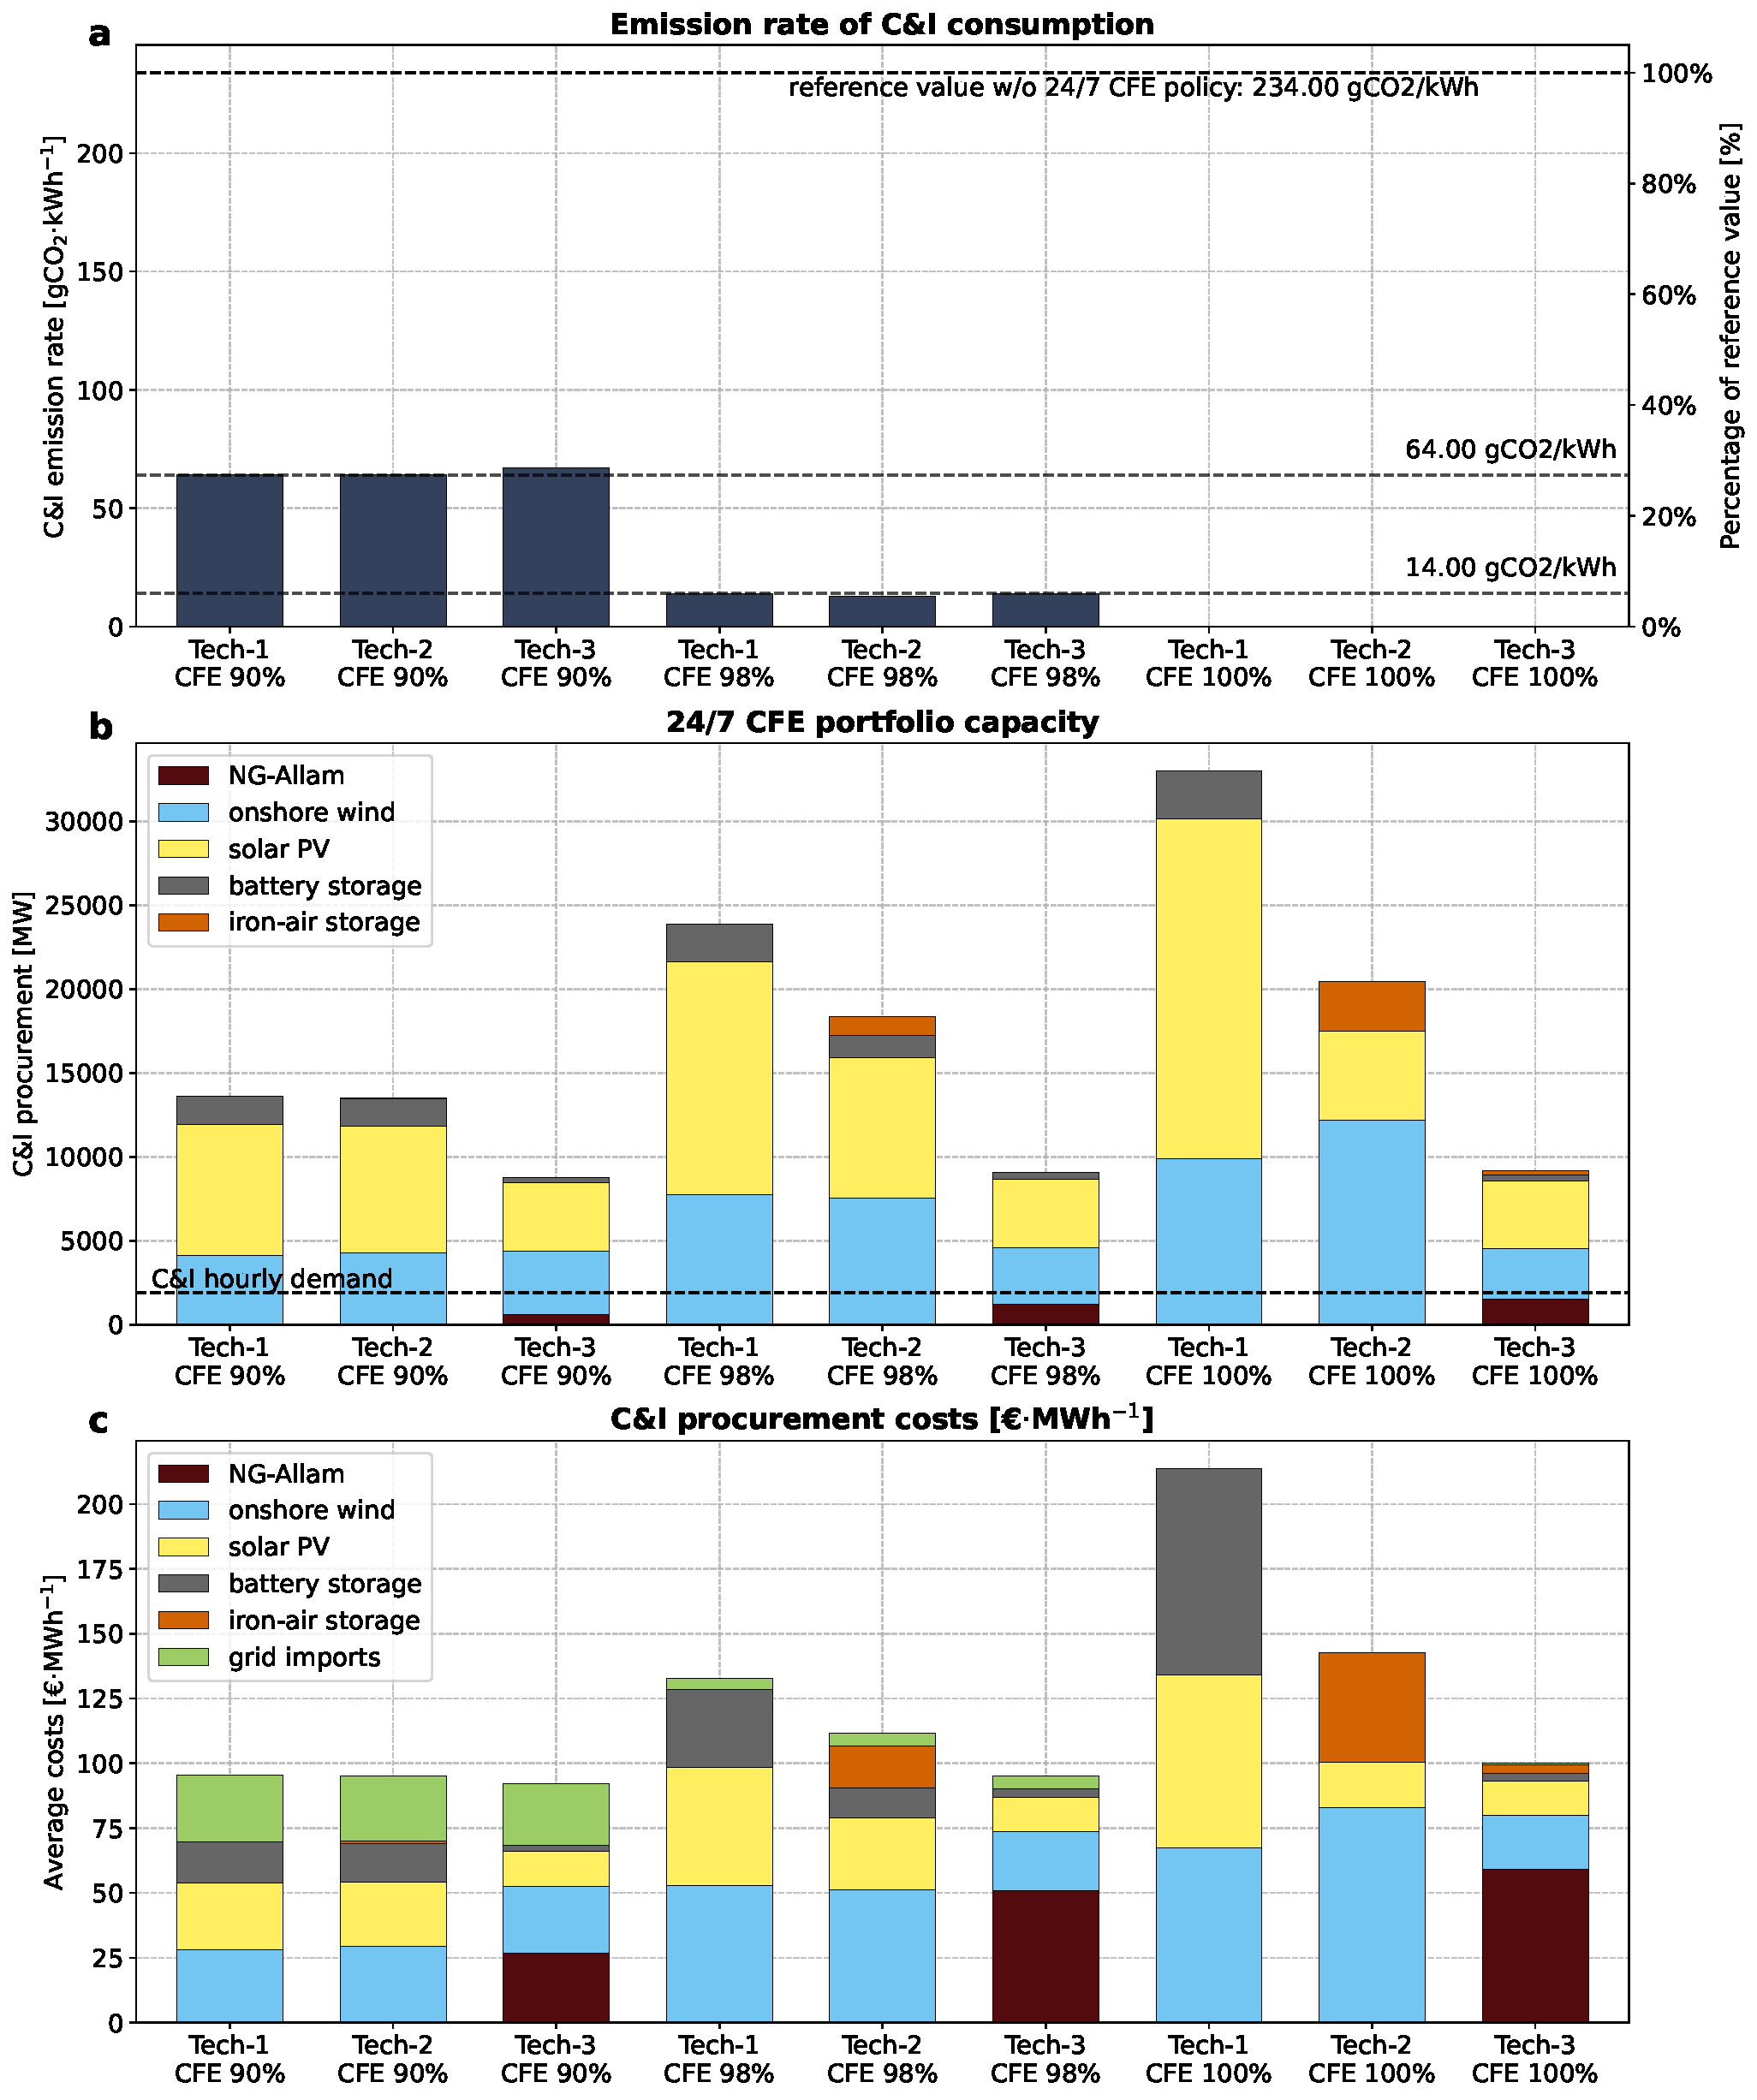
\includegraphics[width=\textwidth]{images/dashboard_247CFE.pdf}
    \captionsetup{width=\textwidth}
    \caption{Illustrative modelling of 24/7 CFE matching.
    \textbf{Panel a}: Average emissions rate of participating consumers,
    \textbf{panel b}: portfolio capacity procured by participating consumers,
    \textbf{panel c}: procurement cost by scenario.
    Here we assume Germany 2025 as an example location and participation rate of C\&I consumers in 24/7 CFE matching strategy at 5\% (ca. 1900~MW load).
    CFE scores 90\%, 98\% and 100\% correspond to the share of time when the electricity consumed by the participating consumers is carbon-free.
    Tech-1: palette of technologies that are commercially available today: onshore wind, utility scale solar PV, and battery storage; Tech-2: all above plus iron-air battery storage; Tech-3: all above plus an Allam cycle generator. The 24/7 CFE procurement framework is based on the methodologies paper by \citet{google-methodologies}. Simulations were carried out using the 24/7 CFE model by \citet{riepinMeansCostsSystemlevel2024}. Technology assumptions are provided in Supplementary Information.\\
    }\label{fig:dashboard}
\end{figure}

\textbf{An illustrative example---} We reproduce the three findings above in an example depicted in Fig. \ref{fig:dashboard}.
Here we display a situation in which a fraction of electricity demand in a particular market bidding zone (here---Germany) voluntarily commits to matching their electricity demand with carbon-free electricity round-the-clock.
Hereinafter, the participating demand is referred to as \enquote{participating consumers}.
\textbf{Panel a} illustrates the intuition---as the CFE target is tightened, participating consumers reduce emission rate (gCO$_2$/kWh$^{-1}$) attributed to their electricity consumption. Once demand and supply are perfectly aligned on an hourly basis, i.e. 100\% 24/7 CFE matching is achieved, participating consumers reach zero emission rate. This goal requires a large portfolio of wind, solar PV, and batteries, as shown in \textbf{panel b}. It is indeed difficult to match every kWh of electricity consumption with renewable electricity during times of dark wind lulls. As a result, achieving 24/7 CFE matching, including the most difficult 2\% of times, adds a high cost premium for consumers in part due the need to overbuild capacity relative to the demand of participating buyers (\enquote{Tech-1, CFE 100\%}). Finding \#3 above is also clearly visible in \textbf{panel c}: the power capacity required for 24/7 CFE matching and associated costs are substantially reduced when LDES technology (iron-air battery storage) or clean firm generation technologies (Allam cycle generator with CCS) are added.

The main observation from Fig. \ref{fig:dashboard} is that 24/7 CFE commitments create an early market for advanced clean electricity technologies, which reduce the costs of hourly CFE matching.
If only 5\% of commercial and industrial (C\&I) consumers in Germany---representing approximately 1900~MW of load---adopt 24/7 CFE matching strategy, this would create a market for approximately 1500~MW of advanced clean firm generators and about 23~GWh of long-duration energy storage (assuming all technology options are deployed,
\enquote{Tech-3, CFE 100\%}).
In a similar vein to how feed-in tariffs and renewable portfolio standards created a \enquote{demand pull} for wind and solar technologies in the past, 24/7 CFE commitments can drive the deployment and accelerate innovation of advanced clean electricity technologies.

\subsection*{Technology learning}\label{sec3}

The early deployment of advanced clean electricity technologies can help them drive down along the \enquote{experience curve} -- a concept encapsulating a set of mechanisms by which technology costs decline as cumulative capacity is deployed: evolving R\&D process, learning-by-doing, incremental upscaling, economies of scale, financial innovation and experience, for example.

In this section, we analyse the expected technological learning for two advanced technologies that can be procured for 24/7 CFE matching: the Allam cycle generator and the iron-air battery storage system.
The mathematical model of learning is based on empirical evidence in which the specific investment costs $C$ of a technology decrease by a constant factor with each doubling of experience $E$ \cite{wayEmpiricallyGroundedTechnology2022a}. The functional dependency is given by:

\begin{equation}
  \begin{aligned}
    \color{violet}C(E)\color{black} &= \color{blue}\overline{C_0}\color{black}  \cdot \left( \frac{\color{red}E}{\color{blue}\overline{E_0}\color{black}} \right)^{-\color{black}\alpha} \text{ where } \color{black}\alpha = \color{black}\log_2 \left( \frac{1}{1 - \color{blue}LR\color{black}} \right)
    \label{eq:learning_curve}
  \end{aligned}
\end{equation}

\noindent where the constants $\color{blue}\overline{C_0}$ [\officialeuro/kW] and $\color{blue}\overline{E_0}$ [MW] are fixed starting points representing the initial costs and experience levels, respectively. The learning rate $\color{blue}LR$ [\%] is a parameter that determines the rate at which costs decrease with experience.
If $\color{blue}LR=20\%$, the costs are reduced by 20\% for each doubling of cumulative experience.
The observed learning rates for energy technologies range from near zero (nuclear, hydropower) to 21\% (daily batteries) \cite{waySuppplementaryMaterialsEmpirically2022}; it is also shown that small, modular energy technologies have advantages to accelerate fast \cite{wilsonGranularTechnologiesAccelerate2020}.
Here we use cumulative capacity $\color{red}E$ [MW] of a technology as a proxy for experience, which is calculated as the sum of the installed capacities of all projects that have been completed by a certain point in time.
We collect information on existing and planned project for each technology, and use this as a starting point for the experience of the technology. 24/7 CFE matching contributes to the technology's experience the additional capacity procured by participating consumers, which is proportional to the participation rate (i.e., the share of electricity demand that is matched with carbon-free electricity on an hourly basis).

The resulting investment costs $\color{violet}C(E)\color{black}$ [\officialeuro/kW] are shown in Fig. \ref{fig:panels} for Allam cycle technology (top panel) and iron-air battery storage (bottom panel).
The first 1\% of participation (around 380~MW load in the German market) reduces costs for Allam cycle generators by 9\% and iron-air storage by 16\%. The technology learning scales significantly from there: at 10\% participation, Allam cycle generators and iron-air storage cost are reduced by 34\% and 45\%, respectively. The learning effect has a diminishing return, due to the logarithmic term $\color{black}\alpha$ in Eq. \ref{eq:learning_curve}. In other words, the first projects have the most significant impact on technology learning, and the effect diminishes as technology experience grows.

The learning model is subject to uncertainty in the initial costs and experience levels, as well as the learning rate. Our Monte Carlo simulation captures this uncertainty by sampling the initial costs and experience levels based on probability distributions derived from public information about planned projects. Fig. \ref{fig:panels} displays the Monte Carlo simulation results as violin plots. Even though both technologies have a wide range of cost outcomes, the main observation is robust to uncertainty: the early deployment of advanced clean electricity technologies due to 24/7 CFE commitments substantially reduces the costs of advanced clean electricity technologies, making them more attractive for other actors and accelerating the point where the technologies become cost-competitive in the rest of the electricity system.

\begin{figure}[htbp]
    \centering
    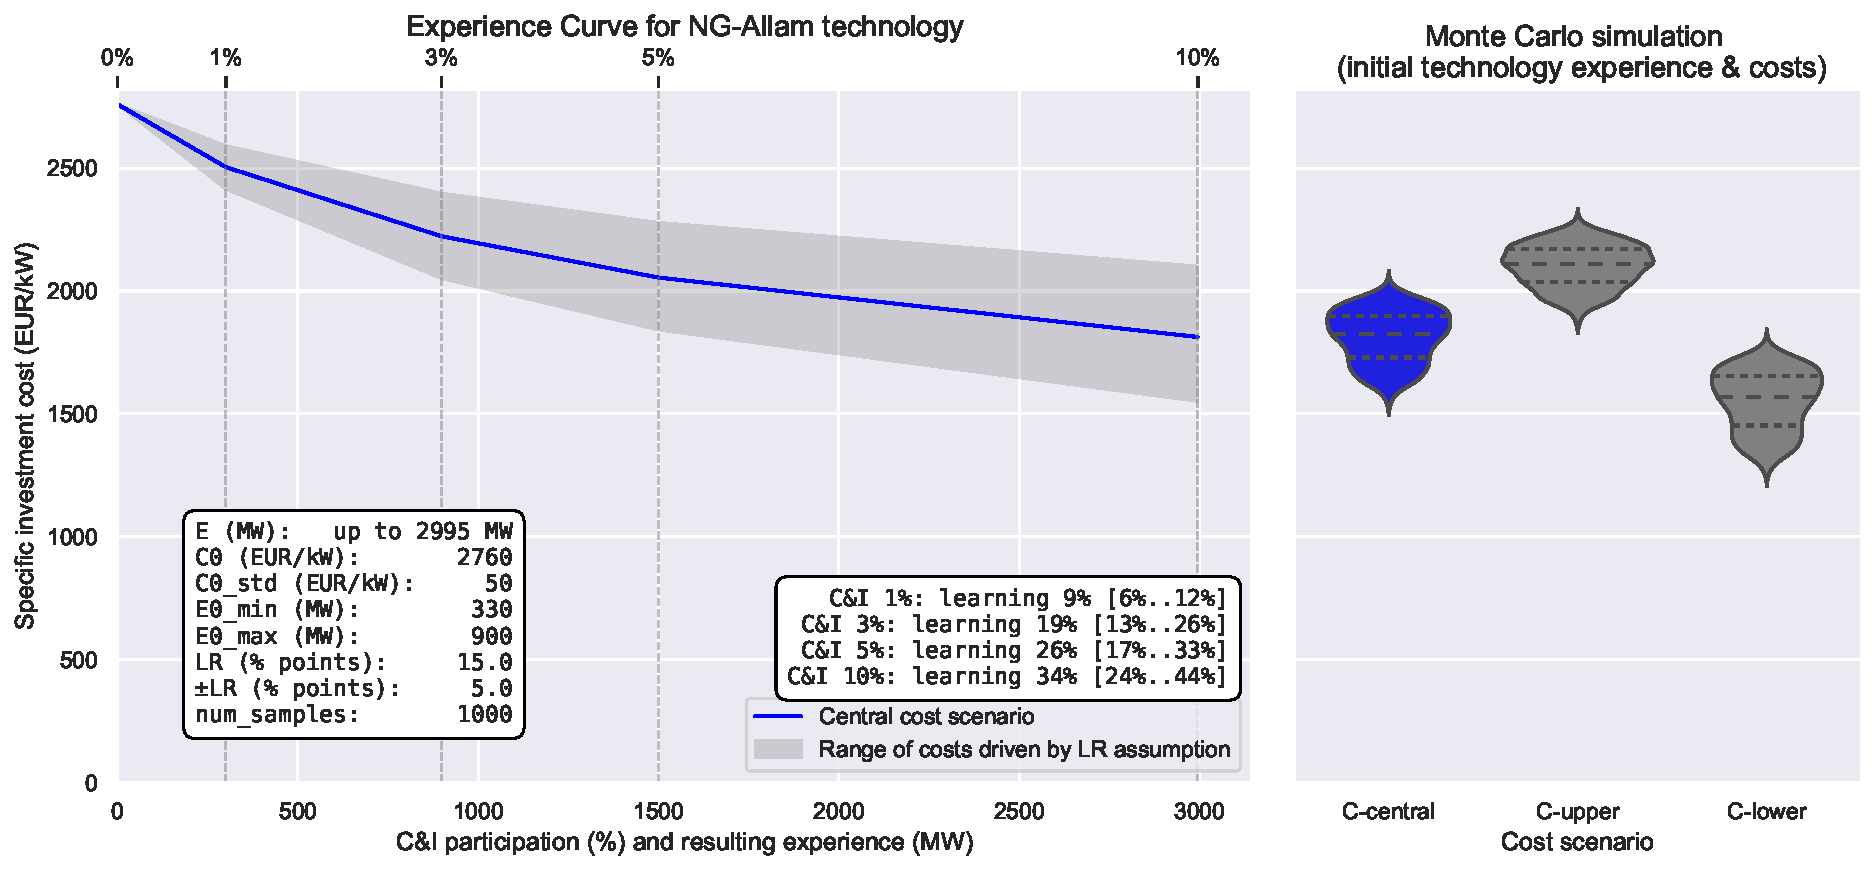
\includegraphics[width=\textwidth]{images/e_curve_NG-Allam.pdf}
    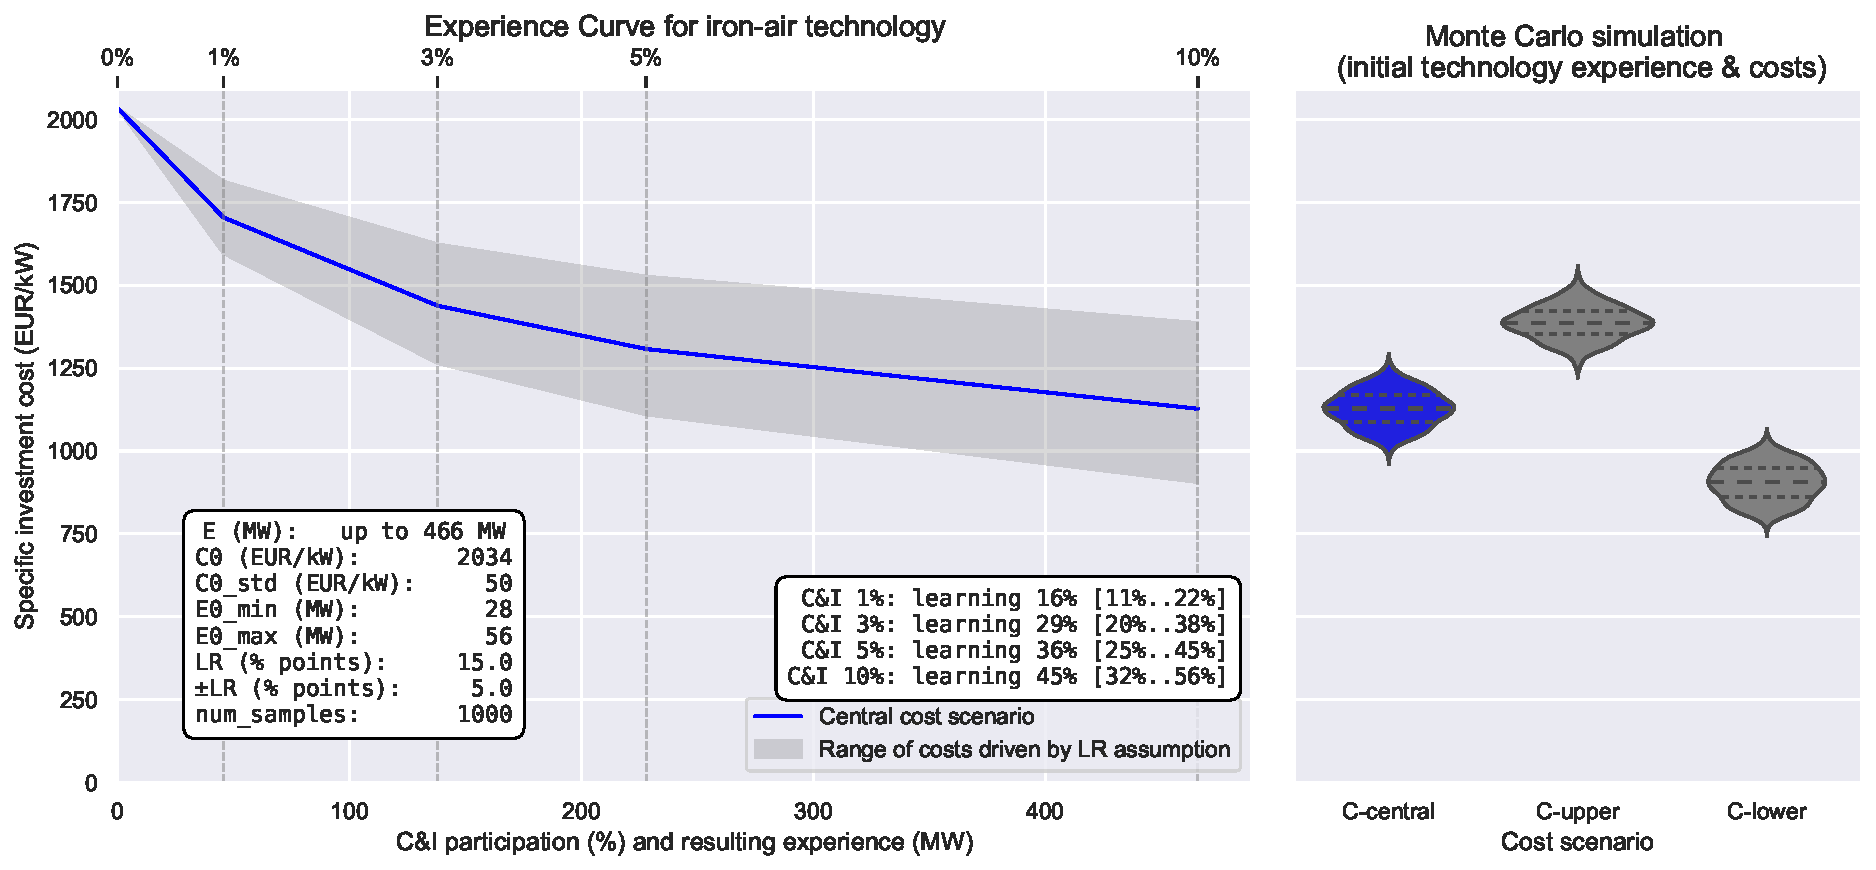
\includegraphics[width=\textwidth]{images/e_curve_iron-air.pdf}
    \caption{Technology learning curves for the NG-Allam cycle (\textbf{top panel}) and iron-air battery storage (\textbf{bottom panel}).
    The learning curves are based on the experience model with the technology investments based on 24/7 CFE model with varying C\&I participation level $[0\%..10\%]$ and learning rates of 15$\pm$5\%.
    For the Monte Carlo analysis calibration, the initial costs (C0) are sampled from a normal distribution with a mean based on technology cost assumptions for 2025 and a standard deviation of 50~EUR/kW. Initial experience levels (E0) are sampled from a uniform distribution, with bounds derived from public information about planned projects. For the NG-Allam case, initial experience lies between cases when one of three planned projects planned by 2025 is completed, and when all three projects are completed (project list is in SI). For the iron-air case, the distribution bounds are formed by assuming that 50\% to 100\% of the projects announced to operate by 2025 are realized on time \cite{FormEnergyLatest2024}.
    }
    \label{fig:panels}
\end{figure}

\subsection*{Beyond directly reduced emissions}\label{sec4}

An illustration of the broader system impact is shown in Fig. \ref{fig:impact}, where we model the German electricity system in 2030 from a system planner's perspective. Here, we minimize the total system costs, including investment costs and operational costs of power generation and storage assets, while adhering to a set of operational constraints. For this case, we assume no voluntary commitments to CFE matching, meaning that power capacity investments are made solely on the basis of economic considerations. The four scenarios represent different levels of CAPEX for iron-air battery storage, starting from the baseline scenario with 2034 \officialeuro/kW, and reducing the cost by 25\% in each step.

The results indicate that iron-air batteries need to cost around 1525 \officialeuro/kW to become economically competitive in the broader electricity system, which represents a 25\% reduction from the baseline. The learning model for iron-air storage shows that this level would require a quadrupling of iron-air capacity expected by 2025 (with a conservative assumption of LR$\sim$12\%, see Fig. \ref{fig:panels}). In other words, assuming that the first movers do not benefit from the learning effect, an investment of approx. \officialeuro340 million (168 [MW] $\cdot$ 2034 [\officialeuro/kW] $\cdot$ 1$^3$ [MW/kW]) can bring iron-air battery storage to the point of economic break-even by 2030, unlocking a wide range of societal benefits. To put this number in perspective, Germany paid approximately \officialeuro 1 billion for redispatch measures only in 2023 \cite{ bnetzaBundesnetzagenturMonitoringberichte2023}; the  costs of the Nord Stream 2 project is estimated at \officialeuro 9.5 billion \cite{cleanenergywireNordStreamSymbol2018}. The unlocked benefits include reduced system emissions---as shown in Fig. \ref{fig:impact}, iron-air storage substitutes fossil peakers (gas open-cycle generators) reducing emissions in the electricity system by 3~MtCO$_2$ annually, already for 25\% reduction in iron-air storage costs. There are other advantages of long-duration storage technology deployment beyond the focus of this analysis, such as reduced curtailment of wind and solar generation, reduced need for additional transmission infrastructure, and increased energy security.

Such learning effect can can be achieved if customers with an aggregate electricity demand of approx. 1200 MW---only 3\% of German C\&I electricity demand---target 24/7 CFE procurement and include iron-air battery storage in their portfolios (see Fig. \ref{fig:panels}). The required investment can be distributed among a wide range of actors since companies from various sectors and regions can join the movement and contribute to technology learning.
Early adoption of advanced technologies will also lead to technology learning and cost reductions for other actors. It spins a \enquote{virtuous circle of innovation}, as we describe next.

\begin{figure}[htbp]
    \centering
    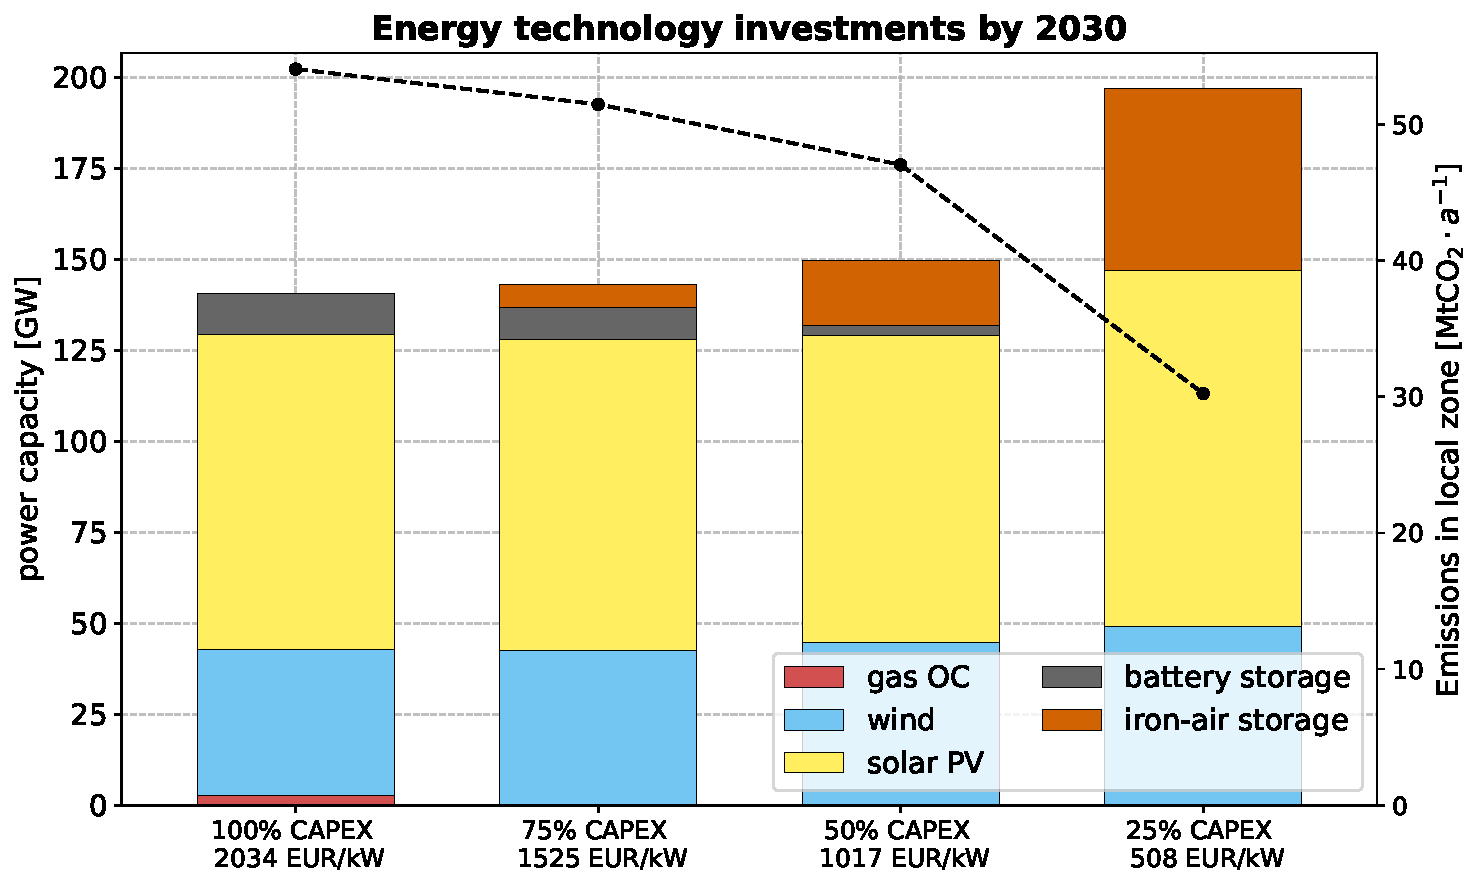
\includegraphics[width=0.8\textwidth]{images/dashboard_3.pdf}
    \caption{Power capacity investments and emissions in German 2030 electricity system as a function of CAPEX for iron-air storage. Here iron-air storage has a fixed duration of 100 hours \cite{FormEnergyLatest2024}. Price for EU ETS allowances is 100 EUR/tCO$_2$. Technology costs are based on DEA \cite{DEA-technologydata}. Other background system assumptions are aligned with \citet{riepinMeansCostsSystemlevel2024}.}\label{fig:impact}
\end{figure}

\subsection*{A virtuous circle of innovation}\label{sec5}

24/7 CFE matching accelerates electricity system decarbonization through three channels: (1) directly reducing emissions during hours with low wind and solar generation, (2) inducing learning effects that make 24/7 matching more attractive for other companies, and (3) enabling these technologies to become cost-competitive and widely adopted across the broader electricity system:

\begin{enumerate}
    \item The first channel comprises two mechanisms for directly reduced emissions. First, \enquote{profile} mechanism refers to participating buyers procuring CFE resources that match their demand patterns. When some consumers align their demand with CFE supply on an hourly basis, the rest of the electricity system requires less dispatchable generation to firm intermittent renewable supply. The utilisation of fossil-based generators, such as gas-fired power plants, is therefore reduced since participating consumers rely on procured CFE resources to cover their demand at all times. This reduces emissions associated with electricity consumption of participating buyers, as shown in Fig. \ref{fig:dashboard}.
    Second, a \enquote{volume} mechanism relates to the impact of excess CFE, i.e., clean electricity generated by 24/7 CFE portfolio that exceeds demand in a given hour can be sold to the grid to replace emitting grid generators. Both mechanisms are explained in detail by \citet{xu-247CFE-report} and \citet{riepinMeansCostsSystemlevel2024}.
    \item Another indirect effect is caused by early commitments to 24/7 CFE that facilitate innovation and create the early market for advanced technologies, as shown in Fig.~\ref{fig:panels}.
    This reduces the price premium for 24/7 CFE procurement goals, encouraging more companies to work towards them. This in turn further lowers system emissions via the two mechanisms in \#1.
    \item Finally, as advanced technologies are deployed repeatedly, they become economically competitive and are adopted more rapidly across the broader electricity system, thereby unlocking greenhouse gas savings beyond the directly reduced emissions associated the corporate portfolios in \#1 and \#2, as shown in Fig. \ref{fig:impact}. This channel is significant as the benefits extend beyond voluntary commitments to clean energy matching, affecting numerous actors in various regions and jurisdictions.
\end{enumerate}

\begin{figure}[h]
    \centering
    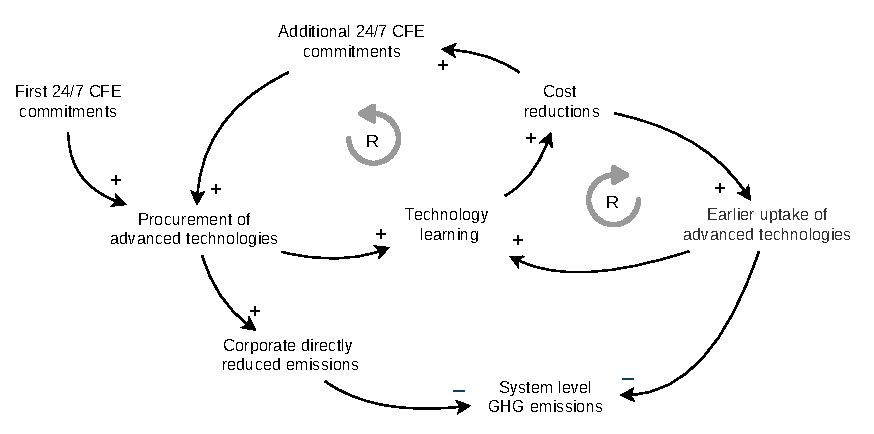
\includegraphics[width=0.9\textwidth]{images/virtuous_dynamics.pdf}
    \caption{System dynamics of 24/7 CFE matching}\label{fig:dynamics}
\end{figure}

Fig. \ref{fig:dynamics} illustrates the nature of the system dynamics that result from initial commitments to 24/7 CFE. It is a self-reinforcing cycle where early commitments create a market for advanced clean electricity technologies, thereby reducing the costs of hourly CFE matching and making more attractive for other companies to join the movement. A second self-reinforcing cycle emerges when advanced clean electricity technologies are adopted early in the electricity system, which further reduces system-level emissions and drives down costs for all actors in the system. The result is a \enquote{virtuous circle} that spurs innovation, financeability, and widespread availability of advanced electricity technologies, thereby accelerating decarbonization of electricity systems.

\subsection*{Takeaways}\label{sec6}

The early market for advanced clean electricity technologies can spur substantial technological learning, leading to cost reductions and unlocking greenhouse gas savings far beyond the reduction of emissions directly associated with initial investments.
The urgency of the climate crisis demands us to expedite this process.
Similarly to the feed-in tariffs and renewable portfolio standards that created a \enquote{demand pull} for wind and solar PV in the past, 24/7 CFE procurement and other advance market commitments \cite{GoogleMicrosoftNucor} accelerate the deployment of advanced clean electricity technologies.
The virtuous system dynamics we describe can be activated by a handful of companies and governments committed to timely action, thereby fostering rapid innovation and making climate solutions more accessible and affordable for everyone.

%%%%%%%%%%%%%%%%%%%%%%%%%%%%%%%%%%%%%%%%%%%%%%%%%%%%%%%%
\backmatter

\bmhead{Acknowledgements} We thank the following people for insights and fruitful discussions: Elisabeth Zeyen, Wilson Ricks, Adam Forni, Brian Denvir, and the participants of the 24/7 CFE Hub Meeting in May 2024. IR and JJ acknowledge a research grant from Google LLC.

\bmhead{Author contributions}
\textbf{Iegor Riepin}: Conceptualization, Methodology, Formal analysis, Writing - Original Draft, Visualization
\textbf{Jesse D. Jenkins}: Conceptualization, Writing - Reviewing and Editing
\textbf{Devon Swezey}: Conceptualization, Writing - Reviewing and Editing
\textbf{Tom Brown}: Conceptualization, Validation, Supervision, Writing - Reviewing and Editing

\bmhead{Code availability} The code to reproduce the illustrative experiments is available at GitHub under open licenses \cite{code247CFE}.

\bmhead{Supplementary Information} Document S1. Table S1: Technology assumptions.Supplementary references.

\bibliography{sn-bibliography}% common bib file
%% if required, the content of .bbl file can be included here once bbl is generated
%%\input sn-article.bbl

\end{document}
